%%%%%%%%%%%%%%%%%%%%% chapter.tex %%%%%%%%%%%%%%%%%%%%%%%%%%%%%%%%%
%
% sample chapter
%
% Use this file as a template for your own input.
%
%%%%%%%%%%%%%%%%%%%%%%%% Springer-Verlag %%%%%%%%%%%%%%%%%%%%%%%%%%
%\motto{Use the template \emph{chapter.tex} to style the various elements of your chapter content.}
%\chapter{Particle accelerators and colliders}
\label{accelerators} % Always give a unique label
% use \chaptermark{}
% to alter or adjust the chapter heading in the running head
\section{Particle accelerators}
We have seen the importance of probing nuclei and particles at high energy. One clear example is given by the weak interactions, where new phenomena (propagator of the interaction) are expected at an energy of the order of $10^5$ MeV. In order to reach high energies, at the beginning  cosmic rays and radioactive sources were used; later on, people started building particle accelerators.

Particle accelerators are extremely complex machines which are based on fundamental, but simple, principles. Those are:
\begin{itemize}
  \item source of particles to be accelerated;
  \item accelerating elements (with electric field);
  \item magnetic elements to bend or focus the beams of particles.
\end{itemize}

\subsection{Electrostatic accelerators}
The simplest particle accelerator is the cathodic tube of Thomson, described in Chapter \ref{Fundamentals-I}. A static electric field, however, is limited by discharging effects. 

The two main static accelerators are:
\begin{enumerate}
    \item \label{item2:Cockroft-Walton} the Cockcroft-Walton accelerator;
    \item \label{item2:Van der Graaf} the Van der Graaf accelerator.
\end{enumerate}

The Cockcroft-Walton accelerator, schematized in Figure \ref{fig:Cockcroft-Walton}, is able to raise a low  alternate current to an high direct voltage trough a system of diodes and capacitors, placed in a tower structure in order to \textit{raise} and \textit{level} the voltage. It is possible to obtain voltages of the order of \SI{1}{MV} and consequently they can be used to accelerate particles to energies of about \SI{1}{MeV}.

\begin{figure}
    \centering
    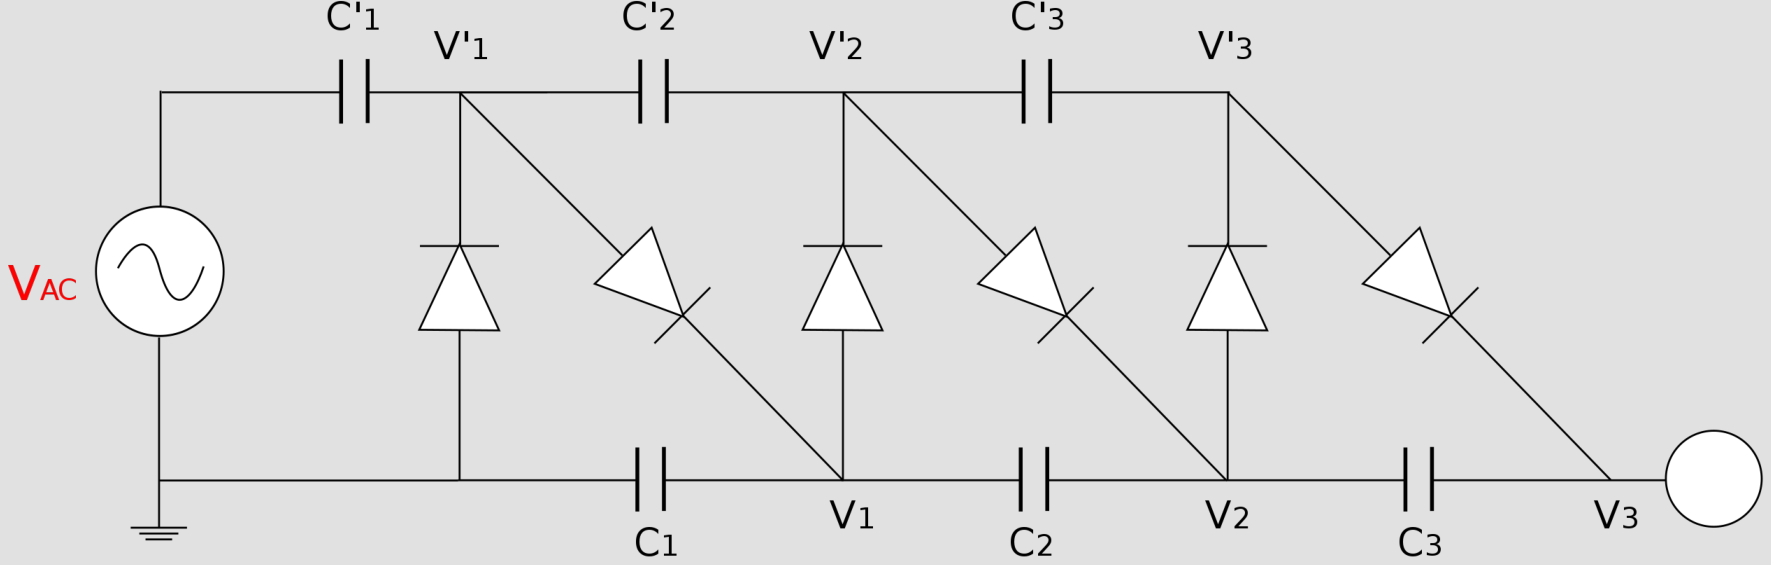
\includegraphics[width=0.8\textwidth]{Figures/Cockcroft-Walton}
    \caption{Schematic view of a Cockcroft-Walton machine. The primed capacitors ($C'$) are the one used to increase the voltage while the other ones are used to level the output of the machine.}
    \label{fig:Cockcroft-Walton}
\end{figure}

The second type of accelerator is the Van der Graaf accelerator. As for the Cockroft-Walton accelerator, this has been developed between 1929 and 1930. Represented in Figure \ref{fig:Van-der-Graaf}, the Van der Graaf accelerator is an electrostatic machine featuring a transport belt (made of insulating cloth) which is used to move the electric charges. The belt, moved by an engine, accumulates the charges onto a conductive sphere which is located in a elevated position in order to isolate the charges from the ground.

In this way it is possible to reach voltages of the order of a few \si{MV}. The highest value ever reached with this kind of machine is \SI{25}{MV}. To go to higher energies new techniques are needed, like for example having particless pass more times through the accelerating fields.

\begin{figure}
    \centering
    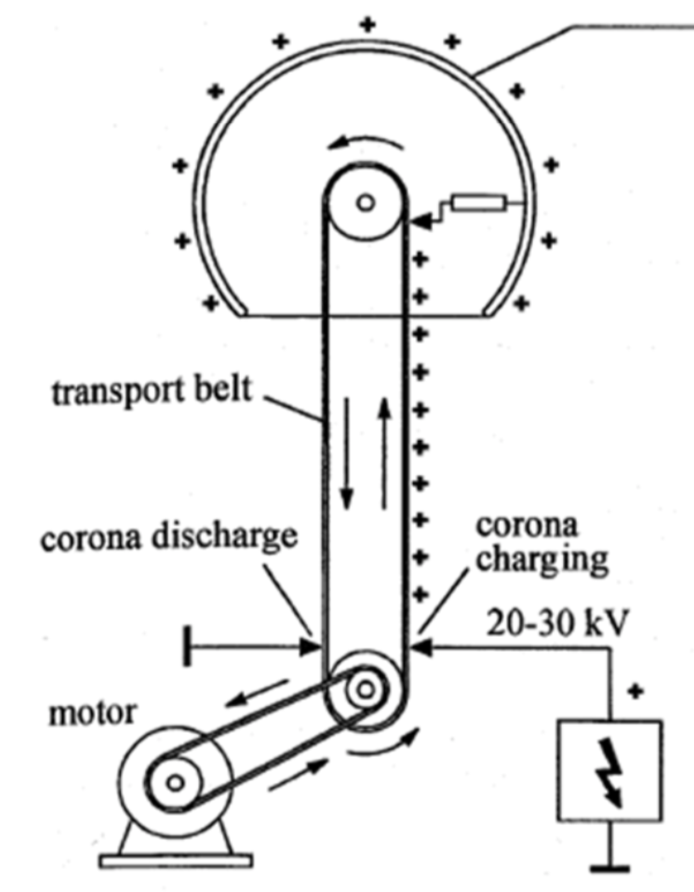
\includegraphics[width=0.3\textwidth]{Figures/Van-der-Graaf}
    \caption{Schematic view of a Van der Graaf generator.}
    \label{fig:Van-der-Graaf}
\end{figure}

\subsection{Wideroe's linear accelerator}
The first linear accelerator featuring an alternated electric field was built by Wideroe (1928) and is represented in Figure \ref{fig:Wideroe-linear-accelerator}. 
\begin{figure}
    \centering
    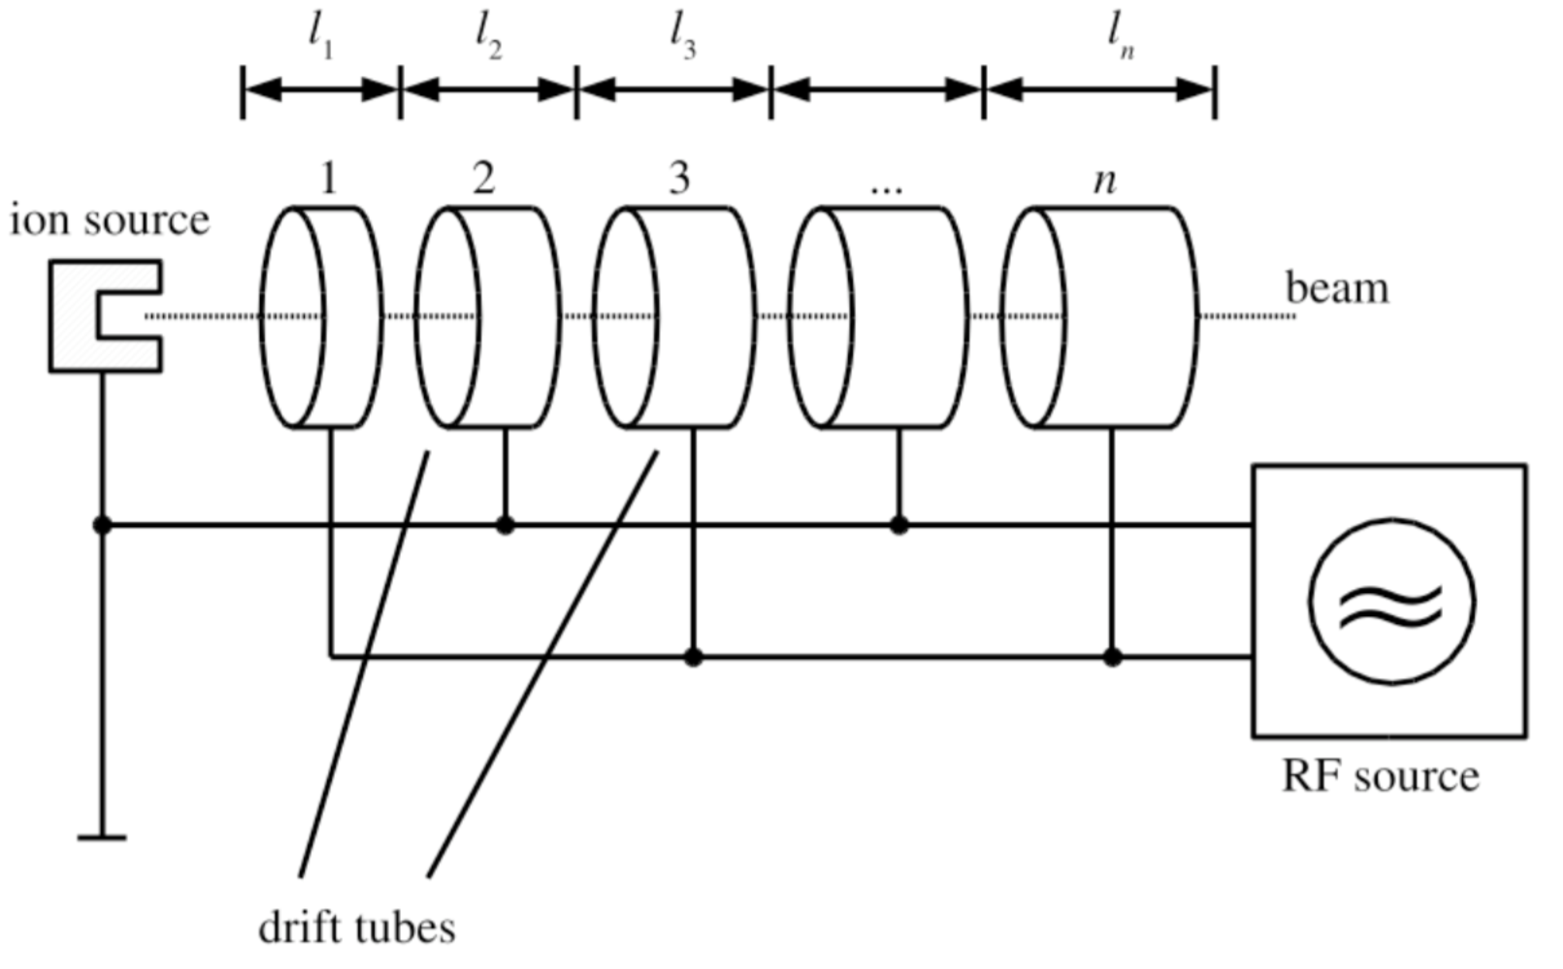
\includegraphics[width=0.6\textwidth]{Figures/Wideroes-linear-accelerator}
    \caption{Schematic of the Wideroe's linear accelerator}
    \label{fig:Wideroe-linear-accelerator}
\end{figure}
In order to accelerate the particles without using high voltages, it is possible to use oscillating voltages built in a way that in each passage the field is in phase with the particles to be accelerated. The path of the particles is fragmented into a series of metallic pipes which act as Faraday's cages. The poles from a single generator are connected in order to invert the voltage of the accelerating fields in the time interval in which the particles goes through the pipe. Increasing lengths of the Faraday's cages, $l_{\small{\text{i}}}$, are chosen, in order to maintain constant the time needed to go trough them, which is the inverse of the frequency of the generator, $t = 1 / f_{RF}$.

\subsection{Cyclotrons}
Another way to achieve multiple passages through an oscillating electric field is adopted in cyclotrons. These machines are circular accelerators in which the frequency of the oscillating field is by construction constant, while the path of particles is controlled by a fixed magnetic field.

The functional principle is obtained equating the Lorentz force to the centripetal acceleration,
\begin{equation}
    qvB = \frac{mv^2}{r},
    \label{eq:cyclotrons}
\end{equation}
where $q$ is the electric charge of the particle, $v$ its velocity, $B$ the magnetic field, $m$ the mass and $r$ the curvature radius.
From Eq. \eqref{eq:cyclotrons}, one immediately obtains
\begin{equation*}
    mv = qBr,
\end{equation*}
so
\begin{equation*}
    r = \frac{mv}{qB}
\end{equation*}
is the curvature radius in a magnetic field. Keeping in mind that the angular velocity is $\omega = \frac{v}{r}$, the rotational frequency is obtained as
\begin{equation*}
    f_{c} = \frac{\omega}{2\pi} = \frac{v}{2\pi r} = \frac{qB}{2\pi m},
\end{equation*}
and does not depend on the radius of the trajectory. As a consequence, it is enough to fix an alternate voltage to obtain, by construction, a synchronisation.

This principle is valid until particles reach the relativistic regime. In this case a correction needs to be applied to the voltage frequency, which becomes
\begin{equation*}
    f = \frac{f_{c}}{\gamma}.
\end{equation*}
This means that the frequency is no more fixed, but must be adjusted during the accelerating procedure. To achieve this, two options are available:
\begin{itemize}
    \item adjust the cyclotron frequency while operating: Cyclo-synchrotrons;
    \item adjust the intensity of the magnetic field: Isosynchronos-cyclotrons - the magnetic field is increased as the radius increases.
\end{itemize}
The first concept of a \SI{9}{in} ($~\SI{23}{cm}$) cyclotron is represented in Fig. \ref{fig:Cyclotron}.
\begin{figure}
    \centering
    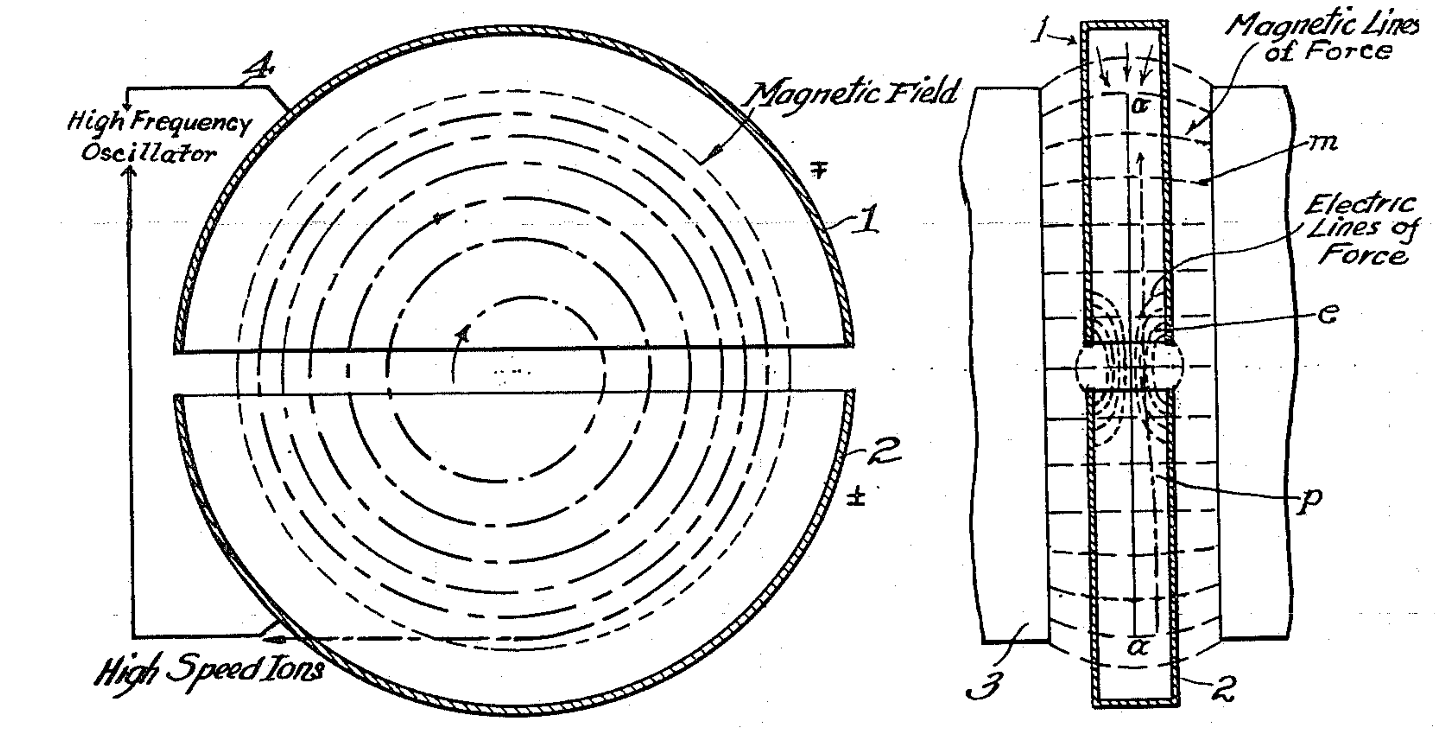
\includegraphics[width=0.8\textwidth]{Figures/Cyclotron}
    \caption{Cyclotron patent from 1931.}
    \label{fig:Cyclotron}
\end{figure}

With simple cyclotrons it was possible to accelerate particles up to \SI{100}{MeV}, while with cyclo-synchrotrons up to \SI{1}{GeV}.

\subsection{Synchrotrons}
The idea of the synchrotron is to have a fixed-radius orbit, in order to be able to build larger machines with the same principle of the linear accelerators: while the electric field is in a decelerating mode, the particles are screened by Faraday's cages. The longitudinal electric field is created by resonant cavities with radio frequencies that produce electromagnetic waves with a longitudinal component which could either accelerate or decelerate charged particles. Therefore, particles need to be synchronised with the machine.

Magnetic elements are used to bend particles in order to constrain them to circular paths. The bending power must increase with higher energies and frequency needs also to be increased in order to maintain synchronisation. An important aspect of the circular motion with fixed radius is that relativistic particles start to loose energy due to irradiation (bremsstrahlung). This plays a central role in setting the maximum achievable energy, and  is related to the kind of particle which is accelerated. In fact, the irradiated power of an accelerated charge with acceleration $a$ and charge $e$ can be expressed as
\begin{equation*}
    W = \frac{1}{6\pi\varepsilon_0c^3}e^2a^2,
\end{equation*}
and taking into account relativistic effects it becomes
\begin{equation*}
    W = \frac{1}{6\pi\varepsilon_0c^3}\gamma^6e^2\left(a^2-\frac{1}{c^2}(\Vec{v}\times\Vec{a})^2\right).
\end{equation*}
For a circular motion of radius $R$, the following relations hold:
\begin{equation*}
    \Vec{v}\times\Vec{a} = va \;\;\;\;\;\text{and}\;\;\;\;\; a = \frac{v^2}{R},
\end{equation*}
therefore the irradiated power can be expressed as 
\begin{equation*}
    W = \frac{e^2}{6\pi\varepsilon_0c^3}\frac{\gamma^4v^4}{R^2}.
\end{equation*}
Using the relation $E = \gamma mc^2$, for $v \rightarrow{c}$ one gets
\begin{equation}
    W = \frac{e^2c}{6\pi\varepsilon_0R^2}\frac{E^4}{(mc^2)^4}.
    \label{eq:irradiated-power}
\end{equation}
Equation \ref{eq:irradiated-power} shows that the irradiated power grows with the fourth power of the energy, and it is inversely proportional to the fourth power of the mass. The irradiated power of an electron is $10^{13}$ times greater than the one of a proton with the same energy.
This energy loss is commonly referred to as \emph{synchrotron radiation}.

For an electron synchrotron, the maximum reachable energy is therefore limited by the maximum acceleration reached in the radio-frequency cavities needed to compensate the energy loss due to irradiation. For a proton synchrotron, instead, the maximum energy is limited by the bending power of the magnets used in the machine, which are needed to maintain the circular orbit. A schematic view of the elements of a synchrotron is shown in Fig. \ref{fig:Synchrotron}, while a picture of the Cosmotron built in Brookhaven is shown in Fig. \ref{fig:Cosmotron}.

\begin{figure}[h]
    \centering
    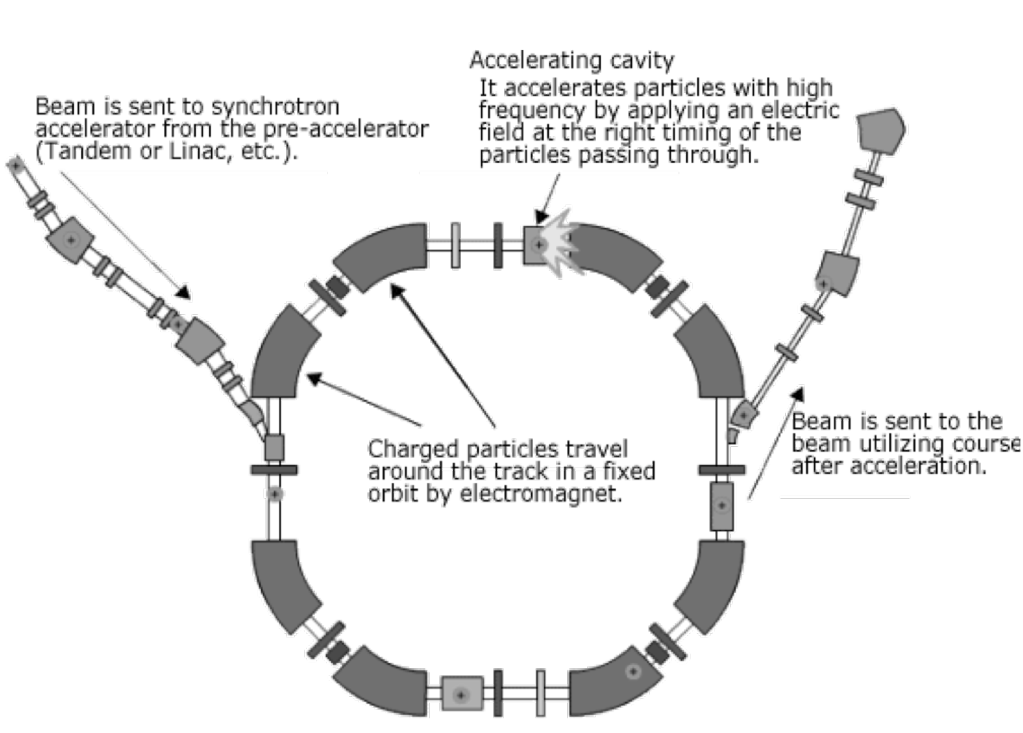
\includegraphics[width=0.75\textwidth]{Figures/Synchrotron}
    \caption{Schematic view of the elements of a synchrotron by V. Kain (CERN).}
    \label{fig:Synchrotron}
\end{figure}
\vspace{3.5cm}
\begin{figure}[h]
    \centering
    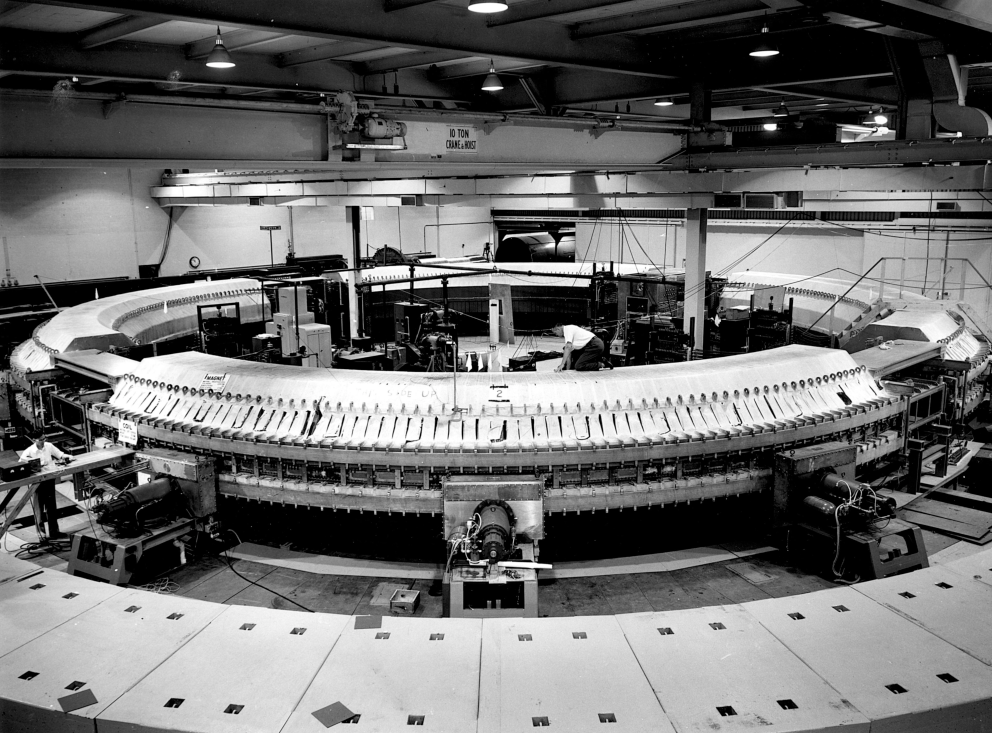
\includegraphics[width=0.65\textwidth]{Figures/Cosmotron}
    \caption{Picture of the Cosmotron, a proton synchrotron which operated at Brookhaven laboratories until 1968.}
    \label{fig:Cosmotron}
\end{figure}
